\subsection{Controller for z axis}
%Derivation of the transfer function 
%
%Root locus and bode
%
%Problem with P controller (Input disturbance)
%
%Simulation of P controller
%
%New controller 
%
%simulation of New controller

It is decided to control the velocity in the z-direction in the inertial system. In order to design such a controller, the transfer function is obtained. The four velocities motor velocities, as input and the velocity in the z-direction in the inertial system, as output.
From \autoref{eq:FinalLinearEquationZ}, with the corresponding translational linearized block diagram in \autoref{fig:TranslationalLinearModelBlockDiagram}, the linear transfer function for the z-direction is readily obtained.
%
\begin{flalign}
  \frac{\dot{Z}_I}{\omega_{sum}} &= \frac{ \frac{1}{4}\ (-2 k_{th})\ \overline{\omega}_{sum} }{ m\ s } & \label{eq:linearTransferFunctionZ}
\end{flalign}

\begin{where}
  \va{\dot{Z}_I}{is the velocity in the z-direction in the inertial system}{}
  \va{\omega_{sum}}{is the sum of velocities to be controlled}{}
  \va{\overline{\omega}_{sum}}{is the sum of rotor velocities in equilibrium}{}
  \va{k_{th}}{is the thrust constant}{}
  \va{m}{is the mass of the quadcopter}{}
\end{where}

This system has a pole in zero and a negative gain, which means that the locus on increasing gain will drive the system into the right half plane and make it unstable. Thus a negative gain is applied as the initial P-controller. If a gain of $-200$ is applied, the controller will bring the velocity to \SI{1}{m \cdot s^{-1}} in approximately \SI{2}{s}, see \autoref{fig:ZstepPcontrolLinear}.

\begin{figure}[H]
	\centering
	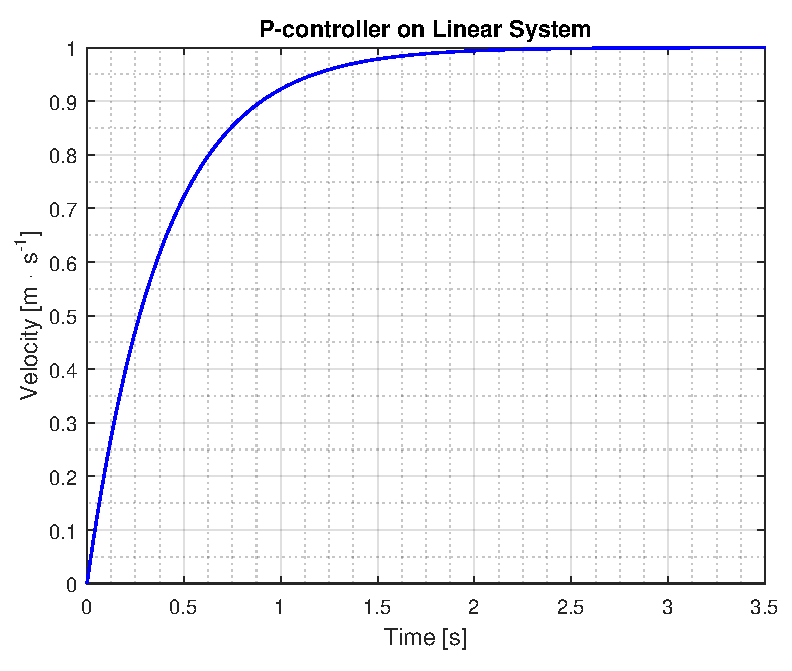
\includegraphics[width=.6\textwidth]{figures/ZstepPcontrolLinear.pdf}
	\caption{Step response of the linear transfer function with a P-controller with a gain of $-200$.}
	\label{fig:ZstepPcontrolLinear}
\end{figure}

However a P-controller does not account for input disturbances, and neither does the integrator in the plant. Therefore, if the equilibrium speed of the rotors has an offset under some flight conditions, this error will not be accounted for.\fxnote{further explanation and formulas are needed here}
To see this effect, the P-controller is tested on the nonlinear model with an added difference of \SI{5}{rad \cdot s^{-1}} in each of the 4 needed equilibrium speeds in the model. The simulation is seen below in \autoref{fig:ZstepPcontrolNonlinear}, where the reference input is subjected to a step of \SI{1}{m \cdot s^{-1}}, however, the velocity stabilizes instead at \SI{0.9}{m \cdot s^{-1}}, revealing a steady state error.

\begin{figure}[H]
	\centering
	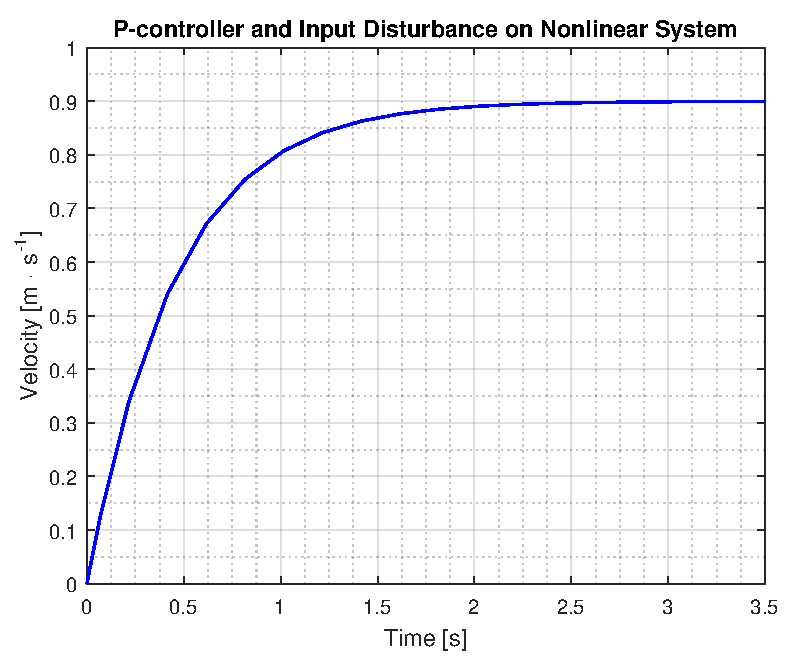
\includegraphics[width=.6\textwidth]{figures/ZstepPcontrolNonlinear.pdf}
	\caption{Step response of the nonlinear transfer function with a P-controller with a gain of $-200$.}
	\label{fig:ZstepPcontrolNonlinear}
\end{figure}

In order to remove the steady state error an integral is introduced to the controller. The root locus of the system, which now contains two poles in zero, will branch along the imaginary axis. To avoid oscillations the two loci are attracted by use of a zero, placed on the left real axis as seen on \autoref{fig:rootLocusOfZwithPI}.

\begin{figure}[H]
	\centering
	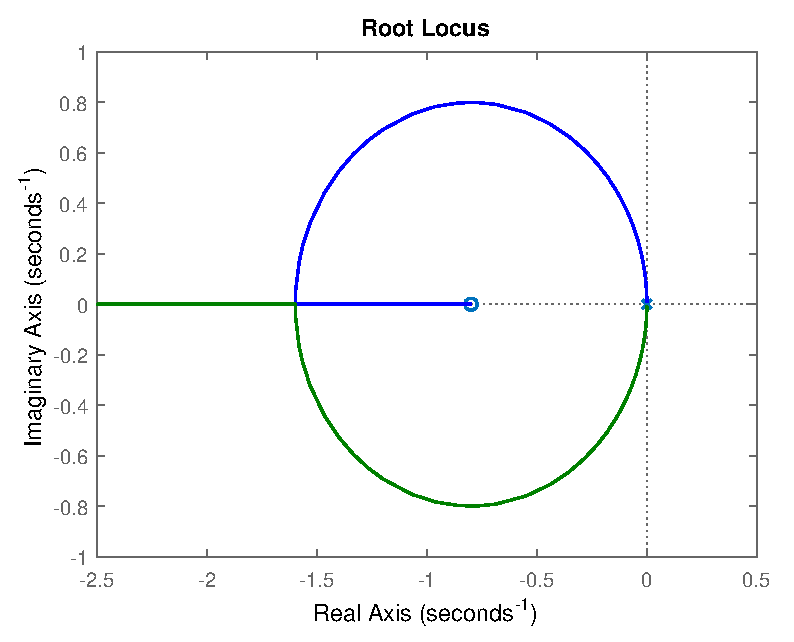
\includegraphics[width=.6\textwidth]{figures/rootLocusOfZwithPI.pdf}
	\caption{Root locus of the system with PI control. The zero is placed in \num{-0.8}.}
	\label{fig:rootLocusOfZwithPI}
\end{figure}

The zero is placed and the gain is scaled to achieve a good rise time with a reasonable control action while still keeping the zero far enough from the poles, such that the integrator is not canceled. The zero is placed in \num{-0.8} and with a gain of \num{-201}. The step response of the linear system with the PI controller is seen on \autoref{fig:stepOfZwithPI}.

\begin{figure}[H]
	\centering
	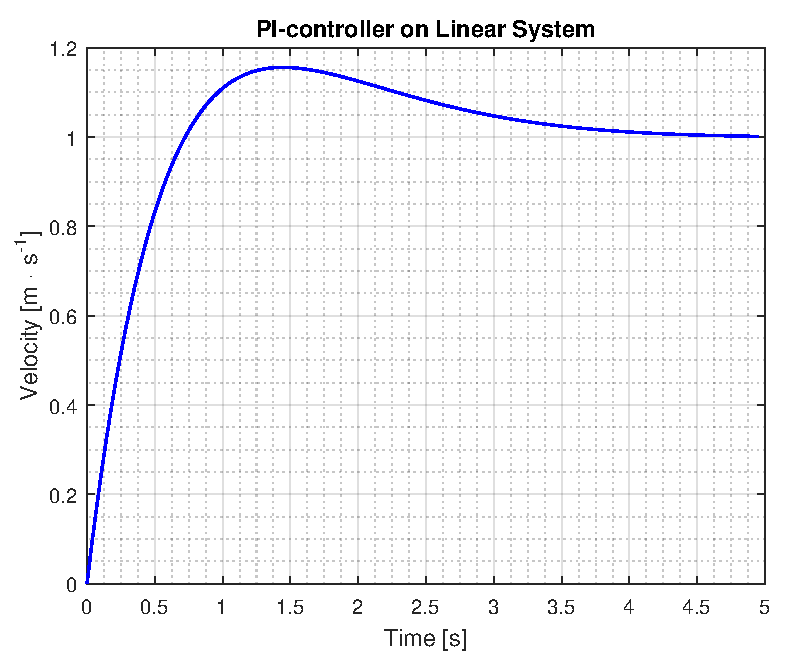
\includegraphics[width=.6\textwidth]{figures/stepOfZwithPI.pdf}
	\caption{Step response of the linear system with PI control.}
	\label{fig:stepOfZwithPI}
\end{figure}

\fxnote{simulation in nonlinear model}

